%---------------------- % % % Personnalisation des couleurs % % % ---------- VERT EMRODE -------
\definecolor{couleurFonce}{RGB}{13,135,119} % Couleur du Code APOGEE
\definecolor{couleurClaire}{RGB}{91,199,185} % Couleur du fond de la bande
\definecolor{couleurTexte}{RGB}{255,255,255} % Couleur du texte de la bande
%------------------------------------------------------------------------------------------


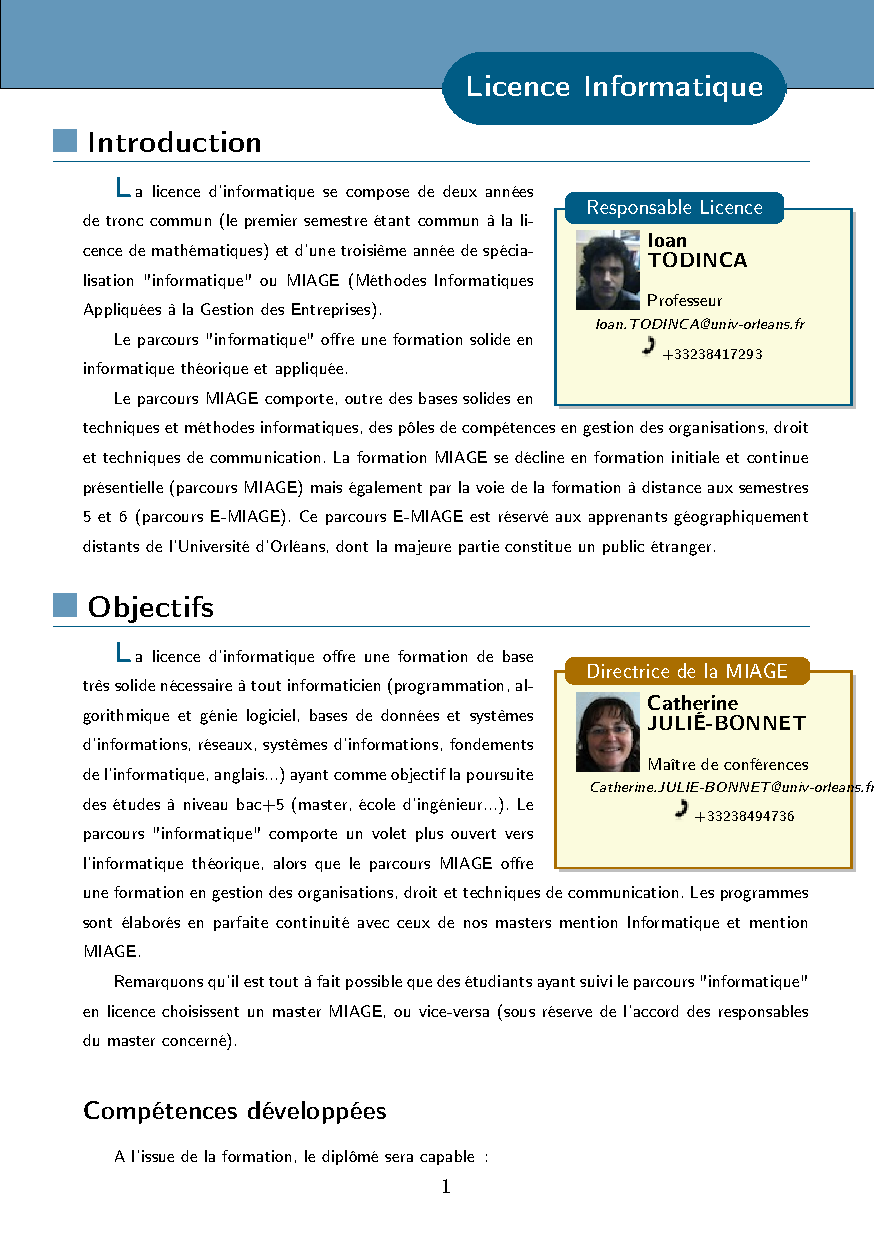
\includepdf[fitpaper,pages=-]{Preambule_Info_MasterINIS_S3S4.pdf}

%==========================================================================================
% Semestre 3
%==========================================================================================

\module[codeApogee={UE 31}, 
titre={Sécurité des applications nomades}, 
CODEUE={1}, 
COURS={20}, 
TD={15}, 
TP={}, 
CTD={}, 
TOTAL={35}, 
SEMESTRE={Semestre 3}, 
COEFF={4}, 
ECTS={4}, 
MethodeEval={Contrôle continue et terminal}, 
ModalitesCCSemestreUn={CC et CT}, 
ModalitesCCSemestreDeux={CT}, 
%CalculNFSessionUne={$\frac{(CC+2*CT)}{3}$}, 
%CalculNFSessionDeux={CT}, 
NoteEliminatoire={7}, 
nomPremierResp={Prénom NOM}, 
emailPremierResp={Prenom.NOM@univ-orleans.fr}, 
nomSecondResp={}, 
emailSecondResp={}, 
langue={Français}, 
nbPrerequis={1}, 
descriptionCourte={true}, 
descriptionLongue={true}, 
objectifs={true}, 
ressources={true}, 
bibliographie={false}] 
{
Unité obligatoire.
} 
{
Ce cours porte sur la sécurité des applications J2ME (Java 2 Mobile Edition) et se décompose en deux parties.
La première partie traite des problèmes liés à la configuration de la politique de sécurité de la machine virtuelle
(security manager, chargeur de classe, contrôle  d\'accès, signature de classes, ...) et des bonnes pratiques de programmation.
Plusieurs aspects du langage Java (héritage, modificateurs,   sérialisation, JNI...) pouvant avoir un impact sur la sécurité des  applications seront étudiés.
En particulier, l\'accent sera mis, au travers d\'une étude de la spécification du langage, sur les pratiques de développement Java conduisant à la production d\'un code robuste.
La seconde partie du cours portera sur le code exécuté par la machine virtuelle et la spécification de cette dernière.
En particulier, les mécanismes de vérification de bytecode mis en oeuvre par la machine virtuelle (principalement basés sur la sureté du typage)
et les techniques d\'analyse sous-jacentes seront étudiés. Finalement, ces techniques d\'analyse seront généralisées afin de permettre
leur application à des propriétés de sécurité plus précises.
} 
{Développement d\'application nomades.
Programmation Java.} 
{\begin{itemize}
\ObjItem Capacité à configurer correctement une machine virtuelle Java en fonction d\'une politique de sécurité donnée.
\ObjItem Maîtrise des subtilités du langage Java ayant un impact sur la sécurité des applications.
\ObjItem Connaissance des propriétés de sureté du code assurées par les machines virtuelle Java et des techniques d\'analyse sous-jacentes.
\ObjItem Application de ces techniques à des propriétés de sécurité spécifiques.
\end{itemize} 
} 
{Ressources} 
{Biblio} 
 
\vfill

%==========================================================================================
\module[codeApogee={UE 32}, 
titre={Système d\'informations géographiques nomades}, 
CODEUE={1}, 
COURS={20}, 
TD={15}, 
TP={}, 
CTD={}, 
TOTAL={35}, 
SEMESTRE={Semestre 3}, 
COEFF={4}, 
ECTS={4}, 
MethodeEval={Contrôle continue et terminal}, 
ModalitesCCSemestreUn={CC et CT}, 
ModalitesCCSemestreDeux={CT}, 
%CalculNFSessionUne={$\frac{(CC+2*CT)}{3}$}, 
%CalculNFSessionDeux={CT}, 
NoteEliminatoire={7}, 
nomPremierResp={Un professionnel du BRGM}, 
emailPremierResp={Bureau de Recherches Géologiques et Minières}, 
nomSecondResp={}, 
emailSecondResp={}, 
langue={Français}, 
nbPrerequis={1}, 
descriptionCourte={true}, 
descriptionLongue={true}, 
objectifs={true}, 
ressources={true}, 
bibliographie={false}] 
{
Unité obligatoire. 
} 
{
\begin{itemize}
\item Apprentissage des principaux systèmes de géo-localisation utilisés dans l\'informatique nomade. Etude des principes et des outils des systèmes d\'informations géographiques (SIG).
\item Analyse des architectures matérielles  et logicielles des SIG nomades.
\end{itemize} 
} 
{Modules de M1 : Système d\'exploitation embarqué, développement d\'applications nomades, réseaux : protocoles et mobilité.} 
{\begin{itemize}
\ObjItem Développer des applications nomades basées sur la géo-localisation et utilisant des SIG.
\end{itemize} 
} 
{Ressources} 
{Biblio} 
 
\vfill

%==========================================================================================
\module[codeApogee={UE 33}, 
titre={Architecture applicatives réparties}, 
CODEUE={1}, 
COURS={20}, 
TD={20}, 
TP={10}, 
CTD={}, 
TOTAL={50}, 
SEMESTRE={Semestre 3}, 
COEFF={4}, 
ECTS={4}, 
MethodeEval={Contrôle continue et terminal}, 
ModalitesCCSemestreUn={CC et CT}, 
ModalitesCCSemestreDeux={CT}, 
%CalculNFSessionUne={$\frac{(CC+2*CT)}{3}$}, 
%CalculNFSessionDeux={CT}, 
NoteEliminatoire={7}, 
nomPremierResp={Frédéric MOAL}, 
emailPremierResp={Frederic.MOAL@univ-orleans.fr}, 
nomSecondResp={Matthieu EXBRAYAT}, 
emailSecondResp={Matthieu.EXBRAYAT@univ-orleans.fr}, 
langue={Français}, 
nbPrerequis={0}, 
descriptionCourte={true}, 
descriptionLongue={true}, 
objectifs={true}, 
ressources={true}, 
bibliographie={false}] 
{
Unité obligatoire. Commune avec le master MIAGE.
} 
{
Ce module se compose de deux parties complémentaires, portant sur les aspects théoriques et pratiques des systèmes d\'information répartis:
\begin{itemize}
\item Concepts et méthodes des SI. Dans cette partie l\'étudiant est sensibilisé aux pratiques modernes des systèmes d\'information,
en vue d\'une prise en charge plus efficace des phases d\'analyse et de conception d\'applications d\'entreprise :
  \begin{itemize}
  \item Typologie des SI et exemples significatifs
  \item UML et processus de développement unifié
  \item Patron de conception (Design Patterns)
  \item Organisation Informatique en entreprise
  \end{itemize} 
\item Concepts et mise en oeuvre des SI répartis. Cette partie est essentiellement articulée autour de la plate forme J2EE.
Dans un premier temps, l\'étudiant se familiarise avec les outils sous-jacents :
  \begin{itemize}
  \item Appel d\'objets répartis via RMI
  \item Echange de messages entre applications distantes via JMS
  \item Persistance d\'objets (utilisation de différents frameworks)
  \item Concept de transaction répartie
  \end{itemize} 
\end{itemize} 
Puis il étudie et met en oeuvre des applications multi-tiers sur une plateforme J2EE :
  \begin{itemize}
  \item Concept de bean métier (EJB)
  \item Intégration des différents types d\'EJB
  \end{itemize}
  De nombreuses manipulations pratiques sont réalisées, en s\'appuyant sur le langage Java (RMI, EJB, Corba, ...).
} 
{Système et répartition.} 
{\begin{itemize}
\ObjItem Fournir les outils nécessaires à l\'analyse, la mise en place et l\'exploitation de systèmes d\'informations répartis.
\ObjItem Apporter une solide formation sur la répartition des données et des traitements dans un Système d\'Information (SI), suivant deux axes :
outils avancés pour la modélisation et la gestion des SI (UML, design patterns, etc.) et SI distribués contemporains (architectures multi-tiers, plateformes applicatives).
\end{itemize} 
} 
{Ressources} 
{Biblio} 
 
\vfill

%==========================================================================================
\module[codeApogee={UE 37}, 
titre={Projet 1}, 
CODEUE={1}, 
COURS={}, 
TD={}, 
TP={}, 
CTD={}, 
TOTAL={}, 
SEMESTRE={Semestre 3}, 
COEFF={3}, 
ECTS={3}, 
MethodeEval={Contrôle continue et terminal}, 
ModalitesCCSemestreUn={Rapport et soutenance de projet}, 
ModalitesCCSemestreDeux={CT}, 
%CalculNFSessionUne={$\frac{(CC+2*CT)}{3}$}, 
%CalculNFSessionDeux={CT}, 
NoteEliminatoire={7}, 
nomPremierResp={Matthieu EXBRAYAT}, 
emailPremierResp={Matthieu.EXBRAYAT@univ-orleans.fr}, 
nomSecondResp={Frédéric DABROWSKI}, 
emailSecondResp={Frederic.DABROWSKI@univ-orleans.fr}, 
nomSecondResp={}, 
emailSecondResp={}, 
langue={Français}, 
nbPrerequis={1}, 
descriptionCourte={true}, 
descriptionLongue={true}, 
objectifs={true}, 
ressources={true}, 
bibliographie={false}] 
{
Unité obligatoire. 
} 
{
Réalisation d\'une application en rapport avec les UE du semestre. 
} 
{Maîtrise des techniques de développement de logiciels.} 
{\begin{itemize}
\ObjItem Mise en pratique des principes et techniques étudiés dans les unités d\'enseignement.
\end{itemize} 
} 
{Ressources} 
{Biblio} 

\vfill

%==========================================================================================
\module[codeApogee={UE 38}, 
titre={Initiation à la recherche}, 
CODEUE={1}, 
COURS={57}, 
TD={}, 
TP={}, 
CTD={}, 
TOTAL={57}, 
SEMESTRE={Semestre 3}, 
COEFF={7}, 
ECTS={7}, 
MethodeEval={Contrôle continue et terminal}, 
ModalitesCCSemestreUn={Rapport et soutenance de projet}, 
ModalitesCCSemestreDeux={CT}, 
%CalculNFSessionUne={$\frac{(CC+2*CT)}{3}$}, 
%CalculNFSessionDeux={CT}, 
NoteEliminatoire={7}, 
nomPremierResp={Matthieu EXBRAYAT}, 
emailPremierResp={Matthieu.EXBRAYAT@univ-orleans.fr}, 
nomSecondResp={Frédéric DABROWSKI}, 
emailSecondResp={Frederic.DABROWSKI@univ-orleans.fr}, 
langue={Français}, 
nbPrerequis={1}, 
descriptionCourte={true}, 
descriptionLongue={true}, 
objectifs={true}, 
ressources={true}, 
bibliographie={false}] 
{
Unité conseillée pour ceux qui se destinent à la recherche.
} 
{
Initiation au stage recherche :
\begin{itemize}
\item introduction d\'outils pour aborder un stage de recherche en laboratoire
\item présentation du cycle de tutoriaux, des thématiques, des possibilités de poursuites en thèse et plus largement du milieu de la recherche académique ou industrielle
\item présentation des projets académiques proposés au semestre 4
\end{itemize} 
Cycle de tutoriaux :
\begin{itemize}
\item 2 tutoriaux longs (d\'une durée totale de 9h; soit 2 fois 3 séances de 1h30) seront axés sur une thématique préalablement
choisie et pour laquelle un renforcement est sollicité par le laboratoire.
\item 20 tutoriaux courts (de 1h30 chacun) articulés autour de thématiques telles que la résolution par contraintes,
l\'apprentissage, extraction de connaissances, le parallélisme, la réalité virtuelle, la sécurité et sûreté des logiciels,
les modèles de calculs, l\'algorithmique et la théorie des graphes, ...
\end{itemize} 
Ces tutoriaux se voudront à la fois introductifs et concrets, mais ils apporteront également des connaissances pointues sur des domaines maîtrisés par les intervenants. 
}
{Avoir une connaissance générale de l\'informatique.}
{\begin{itemize}
\ObjItem L\'objectif est d\'initier l\'étudiant à une démarche scientifique et de le familiariser à un travail de recherche bibliographique. 
\ObjItem Les tutoriaux ont pour objectif d\'appréhender quelques thématiques de recherche et d\'introduire des techniques récentes ou fondamentales.
\end{itemize} 
} 
{Ressources} 
{Biblio} 
 
\vfill

%==========================================================================================
\module[codeApogee={UE 39}, 
titre={Simulation et stratégie d\'entreprise}, 
CODEUE={1}, 
COURS={}, 
TD={24}, 
TP={}, 
CTD={}, 
TOTAL={24}, 
SEMESTRE={Semestre 3}, 
COEFF={3}, 
ECTS={3}, 
MethodeEval={Contrôle continue et terminal}, 
ModalitesCCSemestreUn={CC et CT}, 
ModalitesCCSemestreDeux={CT}, 
%CalculNFSessionUne={$\frac{(CC+2*CT)}{3}$}, 
%CalculNFSessionDeux={CT}, 
NoteEliminatoire={7}, 
nomPremierResp={Chaker HAOUET}, 
emailPremierResp={Chaker.HAOUET@univ-orleans.fr}, 
nomSecondResp={}, 
emailSecondResp={}, 
langue={Français}, 
nbPrerequis={0}, 
descriptionCourte={true}, 
descriptionLongue={true}, 
objectifs={true}, 
ressources={true}, 
bibliographie={false}] 
{
Unité obligatoire. 
} 
{
Les étudiants sont mis en situation de gérer une entreprise à travaers des décisions d\'ordre commercial, financier et de production. Ces entreprises sont en concurrence sur le marché, et sont en mesure d\'évaluer régulièrement leurs résultats à l\'aide des documents financiers et d\'études de positionnement. Ainsi cette situation de gestion d\'entreprise est l\'occasion d\'appliquer les principaux concepts en statégies et marketing, et d\'élaborer des tableaux de bord afin de guider les étudiants dans leurs décisions et d\'en mesurer les impacts financier. 
} 
{} 
{\begin{itemize}
\ObjItem Connaissance du monde de l\'entreprise.
\end{itemize} 
} 
{Ressources} 
{Biblio} 
 
\vfill

%==========================================================================================
\module[codeApogee={UE 34 : WIN}, 
titre={Pratique des contraintes}, 
CODEUE={1}, 
COURS={20}, 
TD={15}, 
TP={}, 
CTD={}, 
TOTAL={35}, 
SEMESTRE={Semestre 3}, 
COEFF={4}, 
ECTS={4}, 
MethodeEval={Contrôle continue et terminal}, 
ModalitesCCSemestreUn={CC et CT}, 
ModalitesCCSemestreDeux={CT}, 
%CalculNFSessionUne={$\frac{(CC+2*CT)}{3}$}, 
%CalculNFSessionDeux={CT}, 
NoteEliminatoire={7}, 
nomPremierResp={Bich DAO}, 
emailPremierResp={Bich.DAO@univ-orleans.fr}, 
nomSecondResp={}, 
emailSecondResp={}, 
langue={Français}, 
nbPrerequis={1}, 
descriptionCourte={true}, 
descriptionLongue={true}, 
objectifs={true}, 
ressources={true}, 
bibliographie={false}] 
{
Unité obligatoire. A choisir pour le parcours WIN : Web, Intelligence et Nomadisme.
} 
{
Ce module s\'inscrit dans une démarche déclarative et descriptive pour modéliser et résoudre des problèmes combinatoires complexes et professionellement pertinents.
On y montre l\'application des contraintes dans un éventail de problèmes réels, en mettant l\'accent sur la pratique de la modélisation et l\'utilisation des outils.
Il s\'inscrit dans la continuité du module PLC de M1 qui présente le paradigme de la programmation logique et offre une introduction aux contraintes. 
} 
{Programmation en logique et par contraintes (vu en M1).} 
{\begin{itemize}
\ObjItem Modélisation et résolution de problèmes par approche déclarative.
\end{itemize} 
} 
{Ressources} 
{Biblio} 
 
\vfill

%==========================================================================================
\module[codeApogee={UE35 : WIN}, 
titre={Webmining et réseaux sociaux}, 
CODEUE={1}, 
COURS={20}, 
TD={15}, 
TP={}, 
CTD={}, 
TOTAL={35}, 
SEMESTRE={Semestre 3}, 
COEFF={4}, 
ECTS={4}, 
MethodeEval={Contrôle continue et terminal}, 
ModalitesCCSemestreUn={CC et CT}, 
ModalitesCCSemestreDeux={CT}, 
%CalculNFSessionUne={$\frac{(CC+2*CT)}{3}$}, 
%CalculNFSessionDeux={CT}, 
NoteEliminatoire={7}, 
nomPremierResp={Matthieu EXBRAYAT}, 
emailPremierResp={Matthieu.EXBRAYAT@univ-orleans.fr}, 
nomSecondResp={}, 
emailSecondResp={}, 
langue={Français}, 
nbPrerequis={0}, 
descriptionCourte={true}, 
descriptionLongue={true}, 
objectifs={true}, 
ressources={true}, 
bibliographie={false}] 
{
Unité obligatoire. A choisir pour le parcours WIN : Web, Intelligence et Nomadisme.
} 
{
\begin{itemize}
\item Fouille dans les réseaux sociaux.
\item Systèmes de recommandation.
\item Données ouvertes.
\item Recherche d\'information.
\end{itemize} 
} 
{} 
{\begin{itemize}
\ObjItem Savoir identifier et explorer intelligemment diverses sources d\'informations offertes par le web. 
\ObjItem Objectif
\end{itemize} 
} 
{Ressources} 
{Biblio} 
 
\vfill

%==========================================================================================
\module[codeApogee={UE 36 : WIN}, 
titre={Extraction de connaissances dans les BD}, 
CODEUE={1}, 
COURS={20}, 
TD={20}, 
TP={10}, 
CTD={}, 
TOTAL={50}, 
SEMESTRE={Semestre 3}, 
COEFF={4}, 
ECTS={4}, 
MethodeEval={Contrôle continue et terminal}, 
ModalitesCCSemestreUn={CC et CT}, 
ModalitesCCSemestreDeux={CT}, 
%CalculNFSessionUne={$\frac{(CC+2*CT)}{3}$}, 
%CalculNFSessionDeux={CT}, 
NoteEliminatoire={7}, 
nomPremierResp={Christel VRAIN}, 
emailPremierResp={Christel.VRAIN@univ-orleans.fr}, 
nomSecondResp={}, 
emailSecondResp={}, 
langue={Français}, 
nbPrerequis={1}, 
descriptionCourte={true}, 
descriptionLongue={true}, 
objectifs={true}, 
ressources={true}, 
bibliographie={false}] 
{
Unité obligatoire. A choisir pour le parcours WIN : Web, Intelligence et Nomadisme. Unité commune avec le master MIAGE.
} 
{
\begin{itemize}
\item Les différents types d\'apprentissage et les différentes tâches 
\item Classification supervisée : arbre de décision, modèles probabilistes, machines à vecteur support, noyaux
\item Evaluation des modèles
\item Classification non supervisée : par partitionnement, hiérarchique, conceptuelle
\item Recherche de règles d\'association 
\end{itemize}
}
{Outils d\'exploration de données, Intelligence Artificielle}
{\begin{itemize}
\ObjItem Utilisation d\'outils : Weka, RapidMiner.
\ObjItem Définir le problème d\'apprentissage : modèle à acquérir, données nécessaires, techniques applicables.
\ObjItem Appliquer des techniques d\'apprentissage.
\end{itemize} 
} 
{Ressources} 
{Biblio} 
 
\vfill

%==========================================================================================
\module[codeApogee={UE 34 : SSL}, 
titre={Sécurité des communications}, 
CODEUE={1}, 
COURS={20}, 
TD={20}, 
TP={}, 
CTD={}, 
TOTAL={40}, 
SEMESTRE={Semestre 3}, 
COEFF={4}, 
ECTS={4}, 
MethodeEval={Contrôle continue et terminal}, 
ModalitesCCSemestreUn={CC et CT}, 
ModalitesCCSemestreDeux={CT}, 
%CalculNFSessionUne={$\frac{(CC+2*CT)}{3}$}, 
%CalculNFSessionDeux={CT}, 
NoteEliminatoire={7}, 
nomPremierResp={Prénom NOM}, 
emailPremierResp={Prenom.NOM@univ-orleans.fr}, 
nomSecondResp={}, 
emailSecondResp={}, 
langue={Français}, 
nbPrerequis={1}, 
descriptionCourte={true}, 
descriptionLongue={true}, 
objectifs={true}, 
ressources={true}, 
bibliographie={false}] 
{
Unité obligatoire. A choisir pour le parcours SSL : Sûreté et Sécurité du Logiciel. Unité commune avec le master MIAGE.
} 
{
Ce module introduit et familiarise les étudiants avec des notions de sécurité relatives aux communications.
Après un survol historique de la compétition perpétuelle entre cryptographie et cryptanalyse, avec comme point clé
la seconde guerre mondiale et le système Enigma, les standards actuels de chiffrements symétriques et asymétriques
sont étudiés en profondeur. Les technologies actuelles permettent des communications synchrones sur des distances
de plusieurs centaines ou milliers de kilomètres. De plus ces communications peuvent contenir des informations
confidentielles et peuvent également nécessiter une authentification des personnes en communication
(communication entre un tiers et un centre de paiement par exemple). Des protocoles de sécurité sont développés
afin de garantir les propriétés mentionnées précédemment. 
Ce module présente les mécanismes d\'authentification,
de confidentialité et d\'intégrité de données et ainsi que quelques protocoles comme Kerberos.
Enfin, le dernier point traité dans ce module démontre que des algorithmes de chiffrement parfaits ne suffisent pas pour garantir
la sécurité d\'un protocole de communication. Les étudiants sont invités à manipuler un outil de simulation et de
vérification de protocoles de sécurité afin de détecter d\'éventuelles failles logiques de conception. 
} 
{Notions de Mathématiques discrètes, réseaux.} 
{\begin{itemize}
\ObjItem Comprendre en profondeur les mécanismes garantissant la sécurité des systèmes et réseaux en thème de
confidentialité, d\'authentification et de disponibilité. 
\ObjItem Modéliser un protocole à partir d\'une spécification textuelle et manipuler un outil de simulation et de vérification.
\end{itemize} 
} 
{Ressources} 
{Biblio} 
 
\vfill

%==========================================================================================
\module[codeApogee={UE 35 : SSL}, 
titre={Sécurité des systèmes d\'exploitation}, 
CODEUE={1}, 
COURS={20}, 
TD={15}, 
TP={}, 
CTD={}, 
TOTAL={35}, 
SEMESTRE={}, 
COEFF={4}, 
ECTS={4}, 
MethodeEval={Contrôle continue et terminal}, 
ModalitesCCSemestreUn={CC et CT}, 
ModalitesCCSemestreDeux={CT}, 
%CalculNFSessionUne={$\frac{(CC+2*CT)}{3}$}, 
%CalculNFSessionDeux={CT}, 
NoteEliminatoire={7}, 
nomPremierResp={Prénom NOM}, 
emailPremierResp={Prenom.NOM@univ-orleans.fr}, 
nomSecondResp={}, 
emailSecondResp={}, 
langue={Français}, 
nbPrerequis={0}, 
descriptionCourte={true}, 
descriptionLongue={true}, 
objectifs={true}, 
ressources={true}, 
bibliographie={false}] 
{
Unité obligatoire. A choisir pour le parcours SSL : Sûreté et Sécurité du Logiciel.
} 
{
\begin{enumerate}
\item 1) Concepts de base sur l\'administration Unix / Windows
  \begin{itemize}
  \item Boot loader et procédure de boot matériel
  \item Les démons et le lancement de services
  \item Les comptes utilisateurs
  \item Le noyau : fonctionnement, modules, configuration et compilation
  \item Les différents types de fichiers
  \end{itemize} 
\item Modèles de sécurité
  \begin{itemize}
  \item Contrôle d\'accès MAC, RBAC, MLS, BLP
  \item Propriétés de sécurité
  \item Séparation de privilèges
  \end{itemize} 
\item Sécurité d\'un système Linux
  \begin{itemize}
  \item Sécurité système : authentification, autorisation, single sign on (LDAP, Kerberos)
  \item Débordements de tampon (buffer overflows)
  \item Surveillance système : Logs, HIDS, Forensics 
  \item Contrôle d\'accès (SELinux, GRSecurity, ...)
  \item Chiffrement de données
  \end{itemize} 
\item Sécurité des systèmes Windows NT
  \begin{itemize}
  \item Principes généraux de sécurité de Windows NT
  \item Active directory
  \item Mécanismes de sécurité niveau système
  \item Sécurité client/serveur de Windows NT
  \item Nouveautés dans Windows 7
  \end{itemize} 
\item Systèmes de détection d\'intrusion
  \begin{itemize}
  \item Principes généraux : Introduction aux IDS
  \item Exploitation des IDS 
  \end{itemize} 
\end{enumerate}
} 
{ Notions de C et programmation shell
- Notions d\'architecture des ordinateurs} 
{\begin{itemize}
\ObjItem Connaître les grands principes de fonctionnement d\'un système d\'exploitation.
\ObjItem Connaître les différents mécanismes permettant de sécuriser un système d\'exploitation.
\ObjItem Acquérir la capacité à administrer un système type UNIX/Windows.
\ObjItem Acquérir la capacité à sécuriser et maintenir la sécurité d\'un système d\'exploitation.
\ObjItem Acquérir la capacité à analyser et rétablir un système compromis.
\end{itemize} 
} 
{Ressources} 
{Biblio} 
 
\vfill

%==========================================================================================
\module[codeApogee={UE 36 : SSL}, 
titre={Qualité et certification}, 
CODEUE={1}, 
COURS={20}, 
TD={15}, 
TP={}, 
CTD={}, 
TOTAL={35}, 
SEMESTRE={Semestre 3}, 
COEFF={4}, 
ECTS={4}, 
MethodeEval={Contrôle continue et terminal}, 
ModalitesCCSemestreUn={CC et CT}, 
ModalitesCCSemestreDeux={CT}, 
%CalculNFSessionUne={$\frac{(CC+2*CT)}{3}$}, 
%CalculNFSessionDeux={CT}, 
NoteEliminatoire={7}, 
nomPremierResp={Prénom NOM}, 
emailPremierResp={Prenom.NOM@univ-orleans.fr}, 
nomSecondResp={}, 
emailSecondResp={}, 
langue={Français}, 
nbPrerequis={0}, 
descriptionCourte={true}, 
descriptionLongue={true}, 
objectifs={true}, 
ressources={true}, 
bibliographie={false}] 
{
Unité obligatoire. A choisir pour le parcours SSL : Sûreté et Sécurité du Logiciel.
} 
{
\begin{enumerate}
\item Qualité logiciel :
  \begin{itemize}
  \item Présentation de la Qualité, historique, bases de la démarche, définitions, coûts, gains, processus
  \item Présentation des normes et référentiels Qualité (ISO 9001, CMM, ISO SPICE), assurance qualité logiciel
  \item Plan d\'assurance de la qualité logicielle
  \item Qualité produit, ISO 9126, métrologie (qualimétrie logicielle), gestion de configuration, gestion des changements
  \item Qualité dans la relation client/fournisseur, MOA/MOE, sous-traitants, tableaux de bord
  \end{itemize} 
\item Certification :
  \begin{itemize}
  \item Systèmes de management du Sysème d\'information
  \item ISO 27000, 2700x et méthode d\'audit (EBIOS, MEHARI, OCTAVE, ITIL, COBIT)
  \item Certifications (audit et organismes)
  \end{itemize} 
\end{enumerate}
} 
{- Architecture des systèmes d\'information 
- Programmation orientée objet} 
{\begin{itemize}
\ObjItem Connaître les différents référentiels qualité.
\ObjItem Connaître les différentes techniques d\'audit.
\ObjItem Savoir mettre en oeuvre une méthode de certification.
\end{itemize} 
} 
{Ressources} 
{Biblio} 
 
\vfill

%==========================================================================================
% Semestre 4
%==========================================================================================

\module[codeApogee={UE 41}, 
titre={Développement avancé d\'applications nomades}, 
CODEUE={1}, 
COURS={20}, 
TD={15}, 
TP={}, 
CTD={}, 
TOTAL={35}, 
SEMESTRE={Semestre 4}, 
COEFF={3}, 
ECTS={3}, 
MethodeEval={Contrôle continue et terminal}, 
ModalitesCCSemestreUn={CC et CT}, 
ModalitesCCSemestreDeux={CT}, 
%CalculNFSessionUne={$\frac{(CC+2*CT)}{3}$}, 
%CalculNFSessionDeux={CT}, 
NoteEliminatoire={7}, 
nomPremierResp={Prénom NOM}, 
emailPremierResp={Prenom.NOM@univ-orleans.fr}, 
nomSecondResp={}, 
emailSecondResp={}, 
langue={Français}, 
nbPrerequis={1}, 
descriptionCourte={true}, 
descriptionLongue={true}, 
objectifs={true}, 
ressources={true}, 
bibliographie={false}] 
{
Unité obligatoire. 
} 
{
Ce module présente les nouvelles ressources embarquées dans les téléphones "nouvelle génération" menant à de nouveaux types d\'applications
communément appelées "applications de réalité augmentée". Le spectre d\'applications imaginables est alors conséquents,
cependant elles doivent respecter un cadre légal. Ainsi, ce cours rappelle également la législation régissant ce type d\'applications.
\begin{enumerate}
\item Présentation des ressources matérielles : Wifi, Bluetooth, capteurs, accéléromètres
\item Description des différentes API selon le support
\item Interactions avec des services WEB
\item Cas d\'étude : un exemple de développement d\'une application "réalité augmentée"
\item Publication des applications 
\end{enumerate}
}
{Développement d\'applications nomades (S2), Sécurité des applications nomades (S3), SIG nomade (S3).} 
{\begin{itemize}
\ObjItem Fournir à l\'étudiant les connaissances matérielles embarquées dans les téléphones "nouvelle génération".
\ObjItem Familiariser l\'étudiant à la programmation d\'application de réalité augmentée. Avoir connaissance du cadre légal régissant ce type d\'applications.
\end{itemize} 
} 
{Ressources} 
{Biblio} 
 
\vfill

%==========================================================================================
\module[codeApogee={UE 42}, 
titre={Web services et interopérabilité}, 
CODEUE={1}, 
COURS={15}, 
TD={15}, 
TP={10}, 
CTD={}, 
TOTAL={40}, 
SEMESTRE={Semestre 4}, 
COEFF={3}, 
ECTS={3}, 
MethodeEval={Contrôle continue et terminal}, 
ModalitesCCSemestreUn={CC et CT}, 
ModalitesCCSemestreDeux={CT}, 
%CalculNFSessionUne={$\frac{(CC+2*CT)}{3}$}, 
%CalculNFSessionDeux={CT}, 
NoteEliminatoire={7}, 
nomPremierResp={Prénom NOM}, 
emailPremierResp={Prenom.NOM@univ-orleans.fr}, 
nomSecondResp={}, 
emailSecondResp={}, 
langue={Français}, 
nbPrerequis={0}, 
descriptionCourte={true}, 
descriptionLongue={true}, 
objectifs={true}, 
ressources={true}, 
bibliographie={false}] 
{
Unité obligatoire. Commune avec le master MIAGE.
} 
{
Ce module permet de comprendre l\'intérêt et les technologies sous-jacentes mises en \oe uvre dans les architectures de type
Services Web (SOAP, WSDL, HTTP, XML...). Le cours magistral présente les technologies et les outils (libres et commerciaux)
et les séances de travaux dirigés sur machines permettent de mettre en pratique les notions présentées en développant deux
SI sous java J2EE et Microsoft .NET qui interopèrent à l\'aide d\'une architecture orientée service. 
} 
{} 
{\begin{itemize}
\ObjItem Comprendre l\'architecture et les technologies sous-jacentes des Services Web, pour permettre l\'interopérabilité entre des systèmes d\'information hétérogènes.
\end{itemize} 
} 
{Ressources} 
{Biblio} 
 
\vfill

%==========================================================================================
\module[codeApogee={UE 43 : WIN}, 
titre={Visualisation avancée de données}, 
CODEUE={1}, 
COURS={20}, 
TD={15}, 
TP={}, 
CTD={}, 
TOTAL={35}, 
SEMESTRE={Semestre 4}, 
COEFF={3}, 
ECTS={3}, 
MethodeEval={Contrôle continue et terminal}, 
ModalitesCCSemestreUn={CC et CT}, 
ModalitesCCSemestreDeux={CT}, 
%CalculNFSessionUne={$\frac{(CC+2*CT)}{3}$}, 
%CalculNFSessionDeux={CT}, 
NoteEliminatoire={7}, 
nomPremierResp={Sébastien LIMET}, 
emailPremierResp={Sebastien.LIMET@univ-orleans.fr}, 
nomSecondResp={}, 
emailSecondResp={}, 
langue={Français}, 
nbPrerequis={1}, 
descriptionCourte={true}, 
descriptionLongue={true}, 
objectifs={true}, 
ressources={true}, 
bibliographie={false}] 
{
Unité obligatoire. A choisir pour le parcours WIN : Web, Intelligence et Nomadisme.
} 
{
La complexité sémantique et la massivité des données issues de mesures scientifiques, de simulations numériques ou
d\'immenses bases de données disponibles sur le réseau, rendent indispensable le recours à la médiation visuelle pour
en permettre une appréhension la plus riche possible.  La mise en oeuvre de  techniques de visualisation élaborées
conduit à utiliser des architectures parallèles et distribués pour faire face à la complexité des traitements numériques
en amont ou propre au rendu visuel. Cette puissance de traitement peut être mise en oeuvre pour simplifier le rendu
afin de l\'adapter à un rendu nomade, mais elle  peut aussi adapter les données en post-traitement pour que celles-ci
soient analysées via un vaste environnement de Réalité Virtuelle multi-écrans plus ou moins distant sur le réseau.
Nous présentons dans ce cours  les fondements du pipeline graphique parallèle, les différentes techniques de rendu
scientifique, les moyens d\'adapter le rendu nomade aux gros volumes de données complexes et enfin nous abordons
la visualisation scientifique utilisant les techniques avancées de Réalité Virtuelle au service de la performance.
} 
{Module Calcul intensif. Module programmation graphique. Notions en Réseaux. Architecture des systèmes.} 
{\begin{itemize}
\ObjItem Comprendre différentes techniques de visualisation d\'information scientifique.
\ObjItem Comprendre le fonctionnement d\'une application graphique nomade.
\ObjItem Aborder sur des exemples les principes des applications  de visualisation scientifique portants sur des données massives de type geo-scientifique ou biologie moléculaire.
\end{itemize} 
} 
{Ressources} 
{Biblio} 
 
\vfill

%==========================================================================================
\module[codeApogee={UE 44 : WIN}, 
titre={Fouille de données et de textes}, 
CODEUE={1}, 
COURS={15}, 
TD={15}, 
TP={10}, 
CTD={}, 
TOTAL={40}, 
SEMESTRE={Semestre 4}, 
COEFF={3}, 
ECTS={3}, 
MethodeEval={Contrôle continue et terminal}, 
ModalitesCCSemestreUn={CC et CT}, 
ModalitesCCSemestreDeux={CT}, 
%CalculNFSessionUne={$\frac{(CC+2*CT)}{3}$}, 
%CalculNFSessionDeux={CT}, 
NoteEliminatoire={7}, 
nomPremierResp={Christel VRAIN}, 
emailPremierResp={Christel.VRAIN@univ-orleans.fr}, 
nomSecondResp={}, 
emailSecondResp={}, 
langue={Français}, 
nbPrerequis={1}, 
descriptionCourte={true}, 
descriptionLongue={true}, 
objectifs={true}, 
ressources={true}, 
bibliographie={false}] 
{
Unité obligatoire. Commune avec le master MIAGE. A choisir pour le parcours WIN : Web, Intelligence et Nomadisme.
} 
{
Cet enseignement permet d\'une part, d\'introduire des techniques importantes, principalement statistiques et bayésiennes,
non présentées dans le module Extraction de Connaissances dans les BD, d\'autre part, d\'élargir la problématique à des
types de données complexes comme les données textuelles.
\begin{enumerate}
\item Algorithme de fouille de données (approfondissement)
  \begin{itemize}
  \item apprentissage statistique (réseaux de neurones, machines à vecteur support, ...)
  \item apprentissage bayésien
  \end{itemize}
\item Extraction de Connaissances à partir de textes 
  \begin{itemize}
  \item Préparation des données
  \item Documents structurés (XML, ...)
  \item Classification de documents 
  \end{itemize}
\end{enumerate}
} 
{Outils pour l\'exploration de données, Extraction de Connaissances dans les Données.} 
{\begin{itemize}
\ObjItem Compléter les connaissances acquises en fouille de données et acquérir de nouvelles compétences sur la fouile de données textuelles. 
\ObjItem Les données textes ont pris une importance croissante avec le développement d\'Internet qui permet de récupérer rapidement des masses de documents.
\ObjItem Il est important d\'avoir des outils permettant de traiter les documents, que ce soit pour la classification,
la recherche d\'informations, la structuration de connaissances sur un domaine, le web sémantique, ...
\end{itemize} 
} 
{Ressources} 
{Biblio} 
 
\vfill

%==========================================================================================
\module[codeApogee={UE 43 : SSL}, 
titre={Réseaux, sécurité et nomadisme}, 
CODEUE={1}, 
COURS={20}, 
TD={15}, 
TP={}, 
CTD={}, 
TOTAL={35}, 
SEMESTRE={Semestre 4}, 
COEFF={3}, 
ECTS={3}, 
MethodeEval={Contrôle continue et terminal}, 
ModalitesCCSemestreUn={CC et CT}, 
ModalitesCCSemestreDeux={CT}, 
%CalculNFSessionUne={$\frac{(CC+2*CT)}{3}$}, 
%CalculNFSessionDeux={CT}, 
NoteEliminatoire={7}, 
nomPremierResp={Prénom NOM}, 
emailPremierResp={Prenom.NOM@univ-orleans.fr}, 
nomSecondResp={}, 
emailSecondResp={}, 
langue={Français}, 
nbPrerequis={1}, 
descriptionCourte={true}, 
descriptionLongue={true}, 
objectifs={true}, 
ressources={true}, 
bibliographie={false}] 
{
Unité obligatoire. A choisir pour le parcours SSL : Sûreté et Sécurité du Logiciel.
} 
{
Protocoles et sécurité:\\
Les attaques réseau. Les méthodes de protection (inetd, tcpwrappers, arp).
Protection des accès distants (PKI, SSO). Switch. VLAN. Routeurs.
Pare-feux, pare-feux applicatifs, proxy.
IPSec, VPN.
SSL, TLS, SSH.
NIDS.
Mobilité dans les réseaux sans fil de type 802.xx:\\
Réseaux mobiles et protocoles IP (IPV6, HMIP, LERS, SIP).
Réseaux mobiles adhoc (par exemple MANET).
Réseaux mobiles de type NEMO (Network Mobility).
Mobilité dans les réseaux téléphoniques:\\
Générations de mobiles (GSM, GPRS, 3G, 3G+, UMTS).
Sécurité des réseaux sans fils:\\
Sécurité des réseaux GSM (authentification et chiffrement, sécurité des cartes SIM, interception d\'appel, sécurité des services de DATA (SMS, MMS)).
Intégrité, confidentialité et disponibilité des données sur les réseaux sans fil (filtrage des adresses MAC, WEP/WPA/WPA2, AAA : Radius, Portail Captif, VPN). 
}
{Réseau (modèle OSI, programmation). Notions de cryptographie.} 
{\begin{itemize}
\ObjItem Découvrir les différents types de réseaux sans fils (IP, GSM, ...).
\ObjItem Connaître les spécificités des réseaux IP sans fils.
\ObjItem Connaître les protocoles de sécurité classiques.
\ObjItem Être capable de sécuriser une architecture réseau pour des applications nomades.
\end{itemize} 
} 
{Ressources} 
{Biblio} 
 
\vfill

%==========================================================================================
\module[codeApogee={UE 44 : SSL}, 
titre={Analyse statique}, 
CODEUE={1}, 
COURS={20}, 
TD={15}, 
TP={}, 
CTD={}, 
TOTAL={35}, 
SEMESTRE={}, 
COEFF={3}, 
ECTS={3}, 
MethodeEval={Contrôle continue et terminal}, 
ModalitesCCSemestreUn={CC et CT}, 
ModalitesCCSemestreDeux={CT}, 
%CalculNFSessionUne={$\frac{(CC+2*CT)}{3}$}, 
%CalculNFSessionDeux={CT}, 
NoteEliminatoire={7}, 
nomPremierResp={Prénom NOM}, 
emailPremierResp={Prenom.NOM@univ-orleans.fr}, 
nomSecondResp={}, 
emailSecondResp={}, 
langue={Français}, 
nbPrerequis={1}, 
descriptionCourte={true}, 
descriptionLongue={true}, 
objectifs={true}, 
ressources={true}, 
bibliographie={false}] 
{
Unité obligatoire. A choisir pour le parcours SSL : Sûreté et Sécurité du Logiciel.
} 
{
La vérification de propriétés dynamiques des programmes, comme par exemple l\'absence d\'accès à des pointeurs nuls, est un problème généralement indécidable.
L\'interprétation abstraite dont traite ce cours fournit un cadre formel et des outils permettant de déterminer des approximations décidables
de ces propriétés pour lesquelles il est possible de dériver des systèmes de type, de vérification et d\'analyse statique.
Ce cours introduit les connaissances nécessaires à la mise oeuvre des techniques d\'interprétation abstraite (théorie des ordres,
théorie des points fixes, connexions de Galois,...). Des exemples concrets d\'utilisation de ces techniques seront étudiés et des outils
d\'analyse statique existants (Frama-C, Astree) seront présentés. 
} 
{Sécurité des Applications Nomades} 
{\begin{itemize}
\ObjItem Connaissances des fondements de l\'analyse statique de programmes.
\ObjItem Capacité à utiliser ces connaissances pour le développement d\'outils de sûreté et de sécurité.
\end{itemize} 
} 
{Ressources} 
{Biblio} 
 
\vfill

%==========================================================================================
\module[codeApogee={UE 45}, 
titre={Projet 2}, 
CODEUE={1}, 
COURS={}, 
TD={}, 
TP={}, 
CTD={}, 
TOTAL={}, 
SEMESTRE={Semestre 4}, 
COEFF={3}, 
ECTS={3}, 
MethodeEval={Contrôle continue et terminal}, 
ModalitesCCSemestreUn={Rapport et soutenance de projet}, 
ModalitesCCSemestreDeux={CT}, 
%CalculNFSessionUne={$\frac{(CC+2*CT)}{3}$}, 
%CalculNFSessionDeux={CT}, 
NoteEliminatoire={7}, 
nomPremierResp={Prénom NOM}, 
emailPremierResp={Prenom.NOM@univ-orleans.fr}, 
nomSecondResp={}, 
emailSecondResp={}, 
langue={Français}, 
nbPrerequis={1}, 
descriptionCourte={true}, 
descriptionLongue={true}, 
objectifs={true}, 
ressources={true}, 
bibliographie={false}] 
{
} 
{
Réalisation d\'une application en rapport avec les UE du semestre. 
} 
{Maîtrise des techniques de développement de logiciels} 
{\begin{itemize}
\ObjItem Mise en pratique de principes et de techniques étudiés dans les unités d\'enseignement. 
\end{itemize} 
} 
{Ressources} 
{Biblio} 
 
\vfill


%==========================================================================================
\module[codeApogee={UE 47}, 
titre={Anglais}, 
CODEUE={1}, 
COURS={}, 
TD={24}, 
TP={}, 
CTD={}, 
TOTAL={24}, 
SEMESTRE={Semestre 4}, 
COEFF={3}, 
ECTS={3}, 
MethodeEval={Contrôle continue et terminal}, 
ModalitesCCSemestreUn={CC et CT}, 
ModalitesCCSemestreDeux={CT}, 
%CalculNFSessionUne={$\frac{(CC+2*CT)}{3}$}, 
%CalculNFSessionDeux={CT}, 
NoteEliminatoire={7}, 
nomPremierResp={Cédric SARRE}, 
emailPremierResp={Cedric.SARRE@univ-orleans.fr}, 
nomSecondResp={}, 
emailSecondResp={}, 
langue={Français}, 
nbPrerequis={1}, 
descriptionCourte={true}, 
descriptionLongue={true}, 
objectifs={true}, 
ressources={true}, 
bibliographie={false}] 
{
Unité obligatoire. 
} 
{
Étude des technique de présentation orale : amélioration de la prononciation, organisation du discours, guidage de l\'auditoire, élaboration d\'aides visuelles. 
} 
{Anglais non professionnel} 
{\begin{itemize}
\ObjItem Savoir négocier des contrats.
\end{itemize} 
} 
{Ressources} 
{Biblio} 
 
\vfill

%==========================================================================================
\module[codeApogee={UE 48}, 
titre={Stage}, 
CODEUE={1}, 
COURS={}, 
TD={}, 
TP={}, 
CTD={}, 
TOTAL={},
SEMESTRE={}, 
COEFF={12}, 
ECTS={12}, 
MethodeEval={Contrôle continue et terminal}, 
ModalitesCCSemestreUn={CC et CT}, 
ModalitesCCSemestreDeux={CT}, 
%CalculNFSessionUne={$\frac{(CC+2*CT)}{3}$}, 
%CalculNFSessionDeux={CT}, 
NoteEliminatoire={7}, 
nomPremierResp={Prénom NOM}, 
emailPremierResp={Prenom.NOM@univ-orleans.fr}, 
nomSecondResp={Alfred HITCHCOCK}, 
emailSecondResp={alfred.hitchcock@univ-orleans.fr}, 
langue={Français}, 
nbPrerequis={0}, 
descriptionCourte={true}, 
descriptionLongue={true}, 
objectifs={true}, 
ressources={true}, 
bibliographie={false}] 
{
Unité obligatoire.
}
{
\begin{itemize}
\item Un stage en entreprise à temps complet de 4 à 6 mois ou
\item Un stage de recherche  à  temps complet de 4 à 6 mois dans un laboratoire au sein d\'une équipe de
recherche confronte l\'étudiant au monde de la recherche et lui permet à  la fois d\'approfondir et d\'individualiser
la formation de base. Bien qu\'il soit conseillé de faire le stage en laboratoire de recherche, le stage peut se dérouler
dans un service de recherche et développement d\'une entreprise.
\end{itemize}
La recherche du stage est à l\'initiative de l\'étudiant.
Cependant, le sujet doit être validé par les responsables de la formation. Le stage fait l\'objet d\'une convention
engageant l\'entreprise ou le laboratoire, l\'université et l\'étudiant.  
} 
{}
{\begin{itemize}
\ObjItem Appliquer tous les concepts vu durant le master.
\end{itemize}
} 
{Ressources} 
{Biblio} 
 
\vfill

%==========================================================================================
\module[codeApogee={UE 46}, 
titre={Préparation au stage recherche}, 
CODEUE={1}, 
COURS={}, 
TD={}, 
TP={}, 
CTD={}, 
TOTAL={}, 
SEMESTRE={Semestre 4}, 
COEFF={6}, 
ECTS={6}, 
MethodeEval={Contrôle continue et terminal}, 
ModalitesCCSemestreUn={Rapport et soutenance de projet}, 
ModalitesCCSemestreDeux={CT}, 
%CalculNFSessionUne={$\frac{(CC+2*CT)}{3}$}, 
%CalculNFSessionDeux={CT}, 
NoteEliminatoire={7}, 
nomPremierResp={Prénom NOM}, 
emailPremierResp={Prenom.NOM@univ-orleans.fr}, 
nomSecondResp={}, 
emailSecondResp={}, 
langue={Français}, 
nbPrerequis={0}, 
descriptionCourte={true}, 
descriptionLongue={true}, 
objectifs={true}, 
ressources={true}, 
bibliographie={false}] 
{
Unité conseillée pour ceux qui se destinent à la recherche.
} 
{
\begin{itemize}
\item Réalisation d\'un état de l\'art ou/et d\'une expérimentation dans un domaine précis de l\'informatique.
\item Initiation à la recherche.
\end{itemize} 
Les étudiants assistent à 4h de cours pour avoir les prérequis pour ce module.
}
{}
{\begin{itemize}
\ObjItem Savoir réaliser un état de l\'art dans un domaine spécialisé de la recherche en informatique et être à même d\'amorcer une démarche scientifique.
\end{itemize} 
} 
{Ressources} 
{Biblio} 
 
\vfill
